In the following problems a number of simple density distributions are 
investigated
that will serve as a reference for models more constrained by 
geophysical observations to be introduced in later sections.
The gravity field can be determined by solving the governing
Poisson equation (\ref{poisson_eqn}) using suitable boundary conditions.
For the special case of spherically symmetric mass distributions
simple 1-D integral expressions can be used to derive the
corresponding radial pressure distribution. 

\vspace{0.5cm}
\fbox{
\begin{minipage}{0.9\textwidth}
\begin{problem}
\label{prob_poisson_homog_sphere}
{\small \it
The internal and external gravity field for a simple model of
a planet can by derived by solving the Poisson equation 
(\ref{poisson_eqn}), and applying appropriate boundary conditions to 
the general solution.
Consider a spherically symmetric planet of radius $R$ and uniform
density $\rho_0$. 

\begin{enumerate}
\item
   Derive expressions for the gravity potential field $U$ and the gravity 
   force field $g = |{\bf g}|$ inside and outside the planet.

   {\it Hints:}
   Solve Poisson's equation in spherical coordinates for the interior $(r \le R)$
   and exterior domain $r \ge R$ separately.
   The separate solutions for the interior $U_{int}, g_{int}$ and  
   exterior $U_{ext}, g_{ext}$ 
   domain each contain two integration constants which can be determined by 
   applying the following boundary conditions,
    \begin{equation}
       \lim_{r \rightarrow \infty} U_{ext}(r) = 0, 
            ~~~ \lim_{r \rightarrow 0} g_{int}(r) < \infty
    \end{equation}

    Continuity of the gravity accelaration $g$ at the surface $r=R$,
    \begin{equation}
       g_{int} (R) = g_{ext} (R)
    \end{equation}

    Continuity of the gravity potential $U$ at the surface $r=R$,
    \begin{equation}
       U_{int} (R) = U_{ext} (R)
    \end{equation}


   {\it Answers}
    \begin{equation}
       g_{int} = \frac{4\pi}{3} G \rho_0 r ~,~~~
       U_{int} = \frac{2\pi}{3} G \rho_0 r^2 - \frac{3}{2} \frac{GM}{R}
    \label{grav_field_unif_sphere_int}
    \end{equation}
    where $M = \frac{4\pi}{3} R^3 \rho_0$ is the planet mass and $G$ is 
    the gravitational constant.

    \begin{equation}
       g_{ext} = \frac{GM}{r^2} ~,~~~
       U_{ext} =   -\frac{GM}{r}
       \label{grav_field_unif_sphere}
    \end{equation}
\item
    Verify that the external gravity force field is identical to the field of a
    concentrated point mass at $r=0$.
    %Derive a corresponding relation between the internal gravity force field and
    %a (different) concentrated point mass, $m(r)$  at the center
    %(see also (\ref{def_equiv_mass1})).
\item
    Derive an expression for the radial distribution of the pressure in the planetary
    interior and compute the central pressure for a case with 
    $\rho_0 = 5.5 \cdot 10^3 \mathrm{kg m^{-3}}$ and
    $R = 6.371 \times 10^6 m$.

    Solution: $P(r) = \frac{2\pi}{3} \rho_0^2 G \left ( R^2 - r^2 \right )$

\end{enumerate}
}
\end{problem}
\end{minipage}
}

\vspace{0.5cm}

The gravity field of a spherically symmetric density
distribution is identical
to the field of an equivalent point-mass.
(see problem \ref{prob_poisson_homog_sphere}  for the spatial case of a uniform density distribution).
This can be formulated as follows,
\begin{equation}
%%U(r) = \int_r^{\infty}g(r') dr'
%%     = - \frac{Gm(r)}{r} ,~~
  g(r) =   \frac{Gm(r)}{r^2},~
\label{def_equiv_mass1}
\end{equation}
with 
\begin{equation}
  m(r) =   \int_{V(r)} \rho dV = 
           \int_0^r \rho(r') 4\pi r'^2 dr'
\label{def_equiv_mass2}
\end{equation}
Here $m(r)$ is the mass inside a sphere of radius $r$ and $g(r)$ is 
the corresponding magnitude of the gravity acceleration.
For the corresponding gravity potential this implies, with
$
\int_r^{\infty} \frac{dU}{dr'} dr' = U(\infty) - U(r) = - U(r)
$,
\begin{equation}
 U(r) = - \int_r^{\infty} \frac{dU}{dr'} dr'
      = \int_r^{\infty} g_r(r') dr'
      = \int_r^{\infty} - g(r') dr'
      = - \int_r^{\infty} \frac{Gm(r')}{r'^2} dr'
\label{equiv_potential}
\end{equation}
where the radial vector component $g_r$ has been expressed in the vector length 
$g$ as $g_r= {\bf g} \cdot {\bf e}_r= - g$.

To derive (\ref{def_equiv_mass1}), the potential field at the 
radial coordinate $r$ 
can be split in contributions originating from an internal- and external density 
distribution $U(r) = U_i (r) + U_e (r)$.
With corresponding pairs, 
$U_i \leftrightarrow \rho_i$, 
and
$U_e \leftrightarrow \rho_e$,
where
$\rho_e(r') = 0, ~r' \le r$,
and
$\rho_e(r') = \rho(r'), ~r' > r$.
This follows from the linearity of the governing Poisson equation.

The field generated by the internal mass distribution is obtained
by integrating the corresponding Poisson equation in spherical 
coordinates,
\begin{equation}
  \frac{1}{r'^2}
  \frac{d}{dr'} r'^2
  \frac{dU_i}{dr'}
   =
  4\pi G \rho_i
\end{equation}
\begin{equation}
  \int_0^r
      \frac{d}{dr'} \left ( r'^2 \frac{dU_i}{dr'} \right ) dr'
   =
  \int_0^r 4\pi G \rho_i r'^2 dr'
\end{equation}
The radial component of the gravity acceleration becomes,
\begin{equation}
   g_r(r) = - \frac{dU_i}{dr} 
          = - \frac{1}{r^2} \int_0^r 4\pi G \rho_i r'^2 dr'
          = - \frac{Gm(r)}{r^2}
\label{eqn_g_rad_comp}
\end{equation}
Furthermore the acceleration field $g_e$ from the external
mass distribution $\rho_e$ for internal evaluation points
$r'<r$ is zero.
The corresponding gravity potential $U_e$ is uniform,
which follows from the relevant Poisson equation,
in spherical coordinates for a spherically symmetric mass distribution,
\begin{equation}
   \frac{1}{r'^2} \frac{d}{dr'} r'^2 \frac{dU_e}{dr'}
    =
   4\pi G \rho_e 
    = 0
   ~\rightarrow~ 
   r'^2 \frac{dU_e}{dr} = A
   ~\rightarrow~ 
   g_e(r') = - \frac{dU_e}{dr'} = -\frac{A}{r'^2}
\end{equation}
A non-singular field requires $A=0,~g_e(r')=0,~r' \le 0$ and,
\begin{equation}
   \frac{dU_e}{dr'} = 0 ~\rightarrow~ U_e(r') = B,~r' \le r
\end{equation}

Looking back at the PREM model, it is a radial model $\rho(r)$ so 
can compute $g_r$ at the surface of the Earth. The code 
is available in /images/prem/ and uses a somewhat naive 
numerical quadrature of Eq.~(\ref{eqn_g_rad_comp}):

\begin{center}
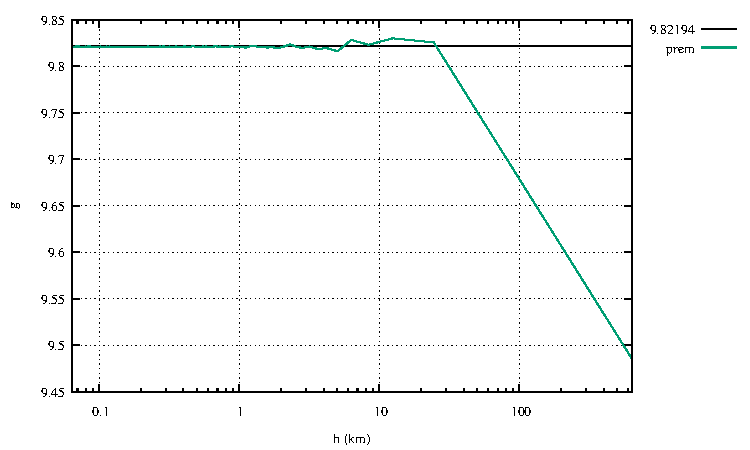
\includegraphics[width=10cm]{images/prem/g.pdf}\\
{\captionfont Radial gravity component measured at the surface
of the Earth as a function of the cell size used for the integration.}
\end{center}




\vspace{0.5cm}
\fbox{
\begin{minipage}{0.9\textwidth}
\begin{problem}
{\small \it
Verify that (\ref{def_equiv_mass1}) and (\ref{equiv_potential}), 
applied to the special case of a homogeneous sphere of density $\rho_0$,
lead to the same expression for the internal and external potential and
acceleration field as given in problem \ref{prob_poisson_homog_sphere}.
}
\end{problem}
\end{minipage}
}

\vspace{0.5cm}

For a two-parameter spherically symmetric planet model consisting of 
a uniform core and mantle with radius $R_c$ and $R_m$ 
and contrasting densities $\rho_c$ and $\rho_m$,
the gravity field can also be determined by solving the
Poisson equation for the particular density distribution and 
determination of the integration constants from the boundary conditions.
However in this case the formula (\ref{def_equiv_mass1}) are more
convenient to obtain expressions for the gravity field.

\vspace{0.5cm}
\fbox{
\begin{minipage}{0.9\textwidth}
\begin{problem}
{\small \it
Derive expressions for the gravity acceleration and internal
pressure distribution for the two-parameter model
\begin{equation}
  \rho(r) =
    \left \{
       \begin{array}{cc}
          \rho_c,   & r < R_c       \\
          \rho_m,   & R_c < r \le R \\
          \rho_e=0, & r > R         \\
       \end{array}
    \right.
  ~,~~
  g(r) =
    \left \{
       \begin{array}{cc}
          g_c, & r < R_c       \\
          g_m, & R_c < r \le R \\
          g_e, & r > R         \\
       \end{array}
    \right.
  ~,~~
  P(r) =
    \left \{
       \begin{array}{cc}
          P_c, & r < R_c  \\
          P_m, & r \ge R_c  \\
       \end{array}
    \right.
\end{equation}
using (\ref{def_equiv_mass1}) and (\ref{def_pressure_integ}).
See also (\ref{pressure_integral}).

{\bf Answer:}
\begin{equation}
  g_c(r) = \frac{4\pi}{3}G \rho_c r
  ,~~
  g_m(r) = \frac{G}{r^2}
           \left \{
             \frac{4\pi}{3} \rho_m 
              \left (
                     r^3 - R_c^3
             \right )
             + M_c
          \right \}
  ,~~
  g_e(r) = \frac{G}{r^2}\left ( M_m + M_c \right )
\end{equation}
\begin{equation}
  M_c = \frac{4\pi}{3} R_c^3 \rho_c 
  ~,~~
  M_m = \frac{4\pi}{3} \rho_m \left ( R^3 - R_c^3 \right )
\end{equation}
\begin{equation}
   P_c(r) = P_m(R_c) + 
            \frac{2\pi}{3} G \rho_c^2 \left ( R_c^2 - r^2 \right )
\end{equation}
\begin{equation}
   P_m(r) = \frac{2\pi}{3} G \rho_m^2 
           \left \{ R_m^2 - r^2 
                    +
                   2 \left (
                       \frac{\rho_c}{\rho_m} -1
                    \right )
                   R_c^3 \left (
                           \frac{1}{r} - \frac{1}{R_m}
                        \right )
          \right \}
\label{eqn_P_2layer_model}
\end{equation}
}
\end{problem}
\end{minipage}
}
